\vspace{-1em}
\section{\protocol/ Protocol}
\vspace{-0.5em}
\label{sec:protocol}

Both fault tolerance and crash consistency mechanisms store redundant data to
correctly recover data from failures. It turns out that \emph{not all
redundancy is necessary} when both mechanisms work together. This observation is the 
ultimate foundation of the \protocol/ protocol. We begin with the
key insights that underly the protocol (\S\ref{ssec:protocol-insight}), 
describe the main steps of the protocol (\S\ref{ssec:protocol-3pu}), and then
determine optimal and safe parameters of
these steps (\S\ref{ssec:protocol-parameters}).

\subsection{Example and Insights}
\vspace{-0.5em}
\label{ssec:protocol-insight}

We derive the insights from discussion of a concrete example.
Hereafter, we keep to the $k$-of-$n$ fault tolerance expression
(\S\ref{ssec:background-ft}), and use \emph{undo logging} to represent
multi-versioning mechanisms (\S\ref{ssec:background-cc}).

\noindent
\textbf{Example.}
Figure~\ref{fig:rain5-compare} shows the write procedure of a log-over-RAID
design and the write procedure of our unified, co-designed approach in RAIN. Both RAID and
RAIN use the same $3/4$ fault tolerance scheme.  Suppose a user writes to
D$_3$. As parity also changes accordingly, both D$_3$ and P need to be updated.
The traditional way is to first log both chunks, as in Step~(1) of (a), and then  update both chunks as in Step~(2).  If any step is
interrupted by a crash, we can {\em always roll back} to the original version.
In each step, chunks can be written in parallel.  Therefore, the total latency
is $2\times$ the latency of a single-chunk write, but the total amount of data
written is $4\times$.

\begin{figure}[!h]
  \centering
  \vspace{-0.5em}
  \includegraphics[width=\linewidth]{figures/RAIN5-compare}
  \caption{Comparison between logging over RAID and
RAIN. D$_n$ denotes a data chunk and P denotes the redundant chunk. Blue chunks
are of the updated version.}
  \vspace{-0.5em}
  \label{fig:rain5-compare}
\end{figure}

\noindent
\textbf{Redundancy.}
Revisiting the procedure, we find that logging can be avoided if data is
recoverable using the parity scheme. Figure~\ref{fig:rain5-compare}(b)
illustrates the refined procedure. In Step~(1), we directly update D$_3$
in-place.  Although this step may corrupt D$_3$ if a crash occurs, the original
version of D$_3$ can be reconstructed from D$_1$, D$_2$, and P, which are all
intact.  Hence, we are able to {\em roll back} to the original version upon a
crash. Then, after D$_3$ has been updated,  P can be updated directly
in-place in Step~(2). If this step is interrupted by a crash, we use
D$_1$, D$_2$, and the already updated D$_3$ to generate the new P.  Therefore, we
can {\em roll forward} to the updated version in case of a crash.  Compared to
the separate log-over-RAID design in (a), the latency of our improved procedure
is the same ($2\times$ the single chunk write latency), but it only writes 2
chunks in total, saving 50\% of the total write size.
This example demonstrates the key idea of co-design that let
us minimize the amount of writes:

\emph{Insight 1 -- If a chunk is recoverable by the fault tolerant scheme (either from
original chunks or updated chunks), that chunk does not need to be logged, thus avoiding extra writes.}

\noindent
\textbf{In-Place Updates.} Another observation from the example is the necessity
of updating chunks in \emph{multiple} phases and executing \emph{different} recovery policies.
In Figure~\ref{fig:rain5-compare}(b), RAIN cannot update D$_3$ and P \emph{in one step},
because the remaining chunks are insufficient to reconstruct the data if a crash corrupts both
D$_3$ and P. Instead, we need two steps as discussed above. The two steps are carefully crafted so that roll-back and roll-forward can be performed, respectively, for recovery. We will see in \S\ref{ssec:protocol-3pu} that three phases are generally necessary, but the basic insight behind the design is as follows.

\emph{Insight 2 -- In-place updates should be done in multiple phases so that: (1)~in an early phase, we can rely on intact chunks to roll back data upon a crash; while (2)~in a late phase, we can rely on already updated chunks to roll forward data upon a crash.}

Note that \protocol/ relies on the capability to distinguish intact,
updated, and corrupted chunks of an ongoing write procedure. To support
such capability, we store \emph{version records} for chunks of an ongoing
procedure. In this section, we focus on demonstration of the protocol; we will
examine the overhead of version records in \S\ref{ssec:rain-meta-overhead}.

\noindent
\textbf{Failure Model.}
The protocol must ensure crash consistency and fault tolerance, or
\emph{safety} for short, in spite of various failures.
In Figure~\ref{fig:rain5-compare}(b), if
one storage node fails \emph{at the same time} as a crash happens,
there would be a risk of data loss. In
Step~(1), if the failure destroys any one of D$_1$, D$_2$ and P,
there would not be sufficiently many intact chunks left to restore the original data after
the crash. The threat to Step~(2) is similar.

Therefore, we need clearly define what scenarios are handled by \protocol/:
a \emph{failure} refers to fail-stop, i.e., a storage node
stops working permanently; a \emph{crash} refers to fail-recover, i.e., the
whole system stops working but then recovers.
% A crash may corrupt data that is being updated.
%Moreover, a user or client failure/crash is acceptable, as the user or client
%always sees atomic updates in the storage.
Since a failure destroys data no matter it is being read or written,
a fault tolerance scheme does \emph{not} distinguish read or write paths.
However, a crash does not affect data in a read path,
but may corrupt data in a write path.
This leads to the following insight.

\emph{
Insight 3 -- When failures and crashes are both taken into account,
we need to differentiate the respective fault tolerance level of read paths and write paths.
}

Specifically, we introduce one more variable $f$
to the $k$-of-$n$ scheme for \protocol/. $f$ is the number of chunk failures our
protocol tolerates during a write path. In contrast, $m$ refers to the number
of failures to tolerate in a read path. Since a crash may bring data damage to a write path, we have $f \le m$.

\vspace{-1em}
\subsection{Three-Phase Update}
\vspace{-0.5em}
\label{ssec:protocol-3pu}

In this section, we convert the insights into the concrete write and recovery procedures of \protocol/.
We first overview the write procedure in a \emph{parameterized}
manner, and then determine and optimize the parameters in
\S\ref{ssec:protocol-parameters}.

\noindent
\textbf{Overview.} Thanks to the fault tolerance scheme, a number of chunks can skip
logging during a write, without violating the crash consistency guarantee.
Those chunks can be updated in-place. \protocol/ performs such in-place updates
in three sequential phases to ensure data safety.

In \emph{Phase~\Romannum{1}}, \protocol/ relies on intact old-version chunks to \emph{roll back}
data upon a crash, as most of the chunks have not yet been updated.  In this
phase, our protocol is supposed to update $s_1$ chunks in-place in parallel. In
the worst case, a crash can corrupt all the $s_1$ chunks; besides,
$f$ failures may happen at the same time. Thus, our protocol chooses $s_1$
such that it is possible to roll back chunks to the old version in the worst
case.

Similarly, when most of the chunks have been updated to the new version, it is
possible  to use the already written new-version chunks for recovery. The final
\emph{Phase~\Romannum{3}} of our protocol updates $s_3$ chunks in-place in parallel
such that if necessary the data can be \emph{rolled forward} to the new version upon a crash
and $f$ simultaneous failures in the worst case.

Between the first and final phase, there is \emph{Phase~\Romannum{2}} in which the number
of old-version chunks and the number of new-version chunks are similar. In this
phase, which version is recoverable depends on the \emph{distribution of failures}.
Figure~\ref{fig:rain1-example} illustrates such a sophisticated case.
It is a three-way replication, i.e., a 1/3 fault
tolerance scheme. We assume tolerance of up to
one failure during the write procedure, so $f = 1$. A write must update all three
chunks. Suppose D is
updated in-place in Phase~\Romannum{1}. It is safe because, even if a crash corrupts D and one failure destroys R$_1$ \emph{or} R$_2$ in the worst case, we can still rely on the remaining chunk to restore the original data.

\begin{figure}[!h]
  \centering
  \vspace{-0.5em}
  \includegraphics[width=0.85\linewidth]{figures/RAIN1-example}
  \caption{The write procedure of \protocol/ with three-way replication
($m = 2$, $f = 1$). A crash and a failure may produce the two states on the
right.}
  \vspace{-0.5em}
  \label{fig:rain1-example}
\end{figure}

Now, we examine Phase~\Romannum{2}. We find that it is safe to in-place update one chunk, e.g., R$_1$.
Suppose a crash corrupts the chunk. Then, a simultaneous failure may result in two
possible states. If the failure
destroys the already updated D, we can roll back using R$_2$; otherwise, if the
failure destroys the original R$_2$, we can roll forward using D. The recovery
policy depends on where the failure happens, i.e., the distribution of the failure(s).
In \S\ref{ssec:protocol-parameters}, we will employ a mathematical method to
show that, no matter how failures are distributed,
\emph{either} roll-back \emph{or} roll-forward is applicable as long as the
number of chunks updated in parallel is limited to a small number $\epsilon$.
Finally, we can in-place update one chunk in-place in Phase~\Romannum{3} whose recovery policy is always roll-forward.

\noindent
\textbf{Parameterized Algorithm.} The pseudo-code in Algorithm~\ref{alg:write} describes the above procedure.  
We consider a stripe of $n$
chunks using a $k$-of-$n$ fault tolerance scheme. A write request modifies $u$ chunks
(including the $m$ redundant chunks). A
traditional logging method has to duplicate all $u$ chunks, while our procedure
allows $\delta$ chunks to be updated in-place, saving $\delta$ chunk writes.

\begin{algorithm}[!t]
\caption{Write procedure of \protocol/ (for one stripe).}
\label{alg:write}
\begin{algorithmic}[1]
  \Require $u$, the number of chunks to update in the stripe; $\delta$, the
number of chunks to avoid logging; $s_1$, max \# of chunks to update in
Phase~\Romannum{1}; $\epsilon$, max \# of chunks to update in one step of
Phase~\Romannum{2}; $s_3$, max \# of chunks to update in Phase~\Romannum{3}.
  \State Log $u - \delta$ chunks and update them \label{alg:log}
  \State Update $s_1$ chunks in-place in parallel \Comment{
\textcolor{brown}{\small Phase~\Romannum{1}}} \label{alg:p1}
  \If {$\delta > s_1 + s_3$}
    \State $s_2 \gets \delta - s_1 - s_3$ \Comment{
\textcolor{brown}{\small \# of updates in Phase~\Romannum{2}}} \label{alg:s2}
    \State $i \gets 0$ \label{alg:p2-begin}
	\While{$i < s_2$} \Comment{ \textcolor{brown}{\small Phase~\Romannum{2}}}
	  \State Update $\epsilon$ chunks in-place in parallel
      \State $i \gets i + \epsilon$
    \EndWhile \label{alg:p2-end}
  \EndIf
  \State Update the rest chunks (up to $s_3$) in-place in parallel \Comment{
\textcolor{brown}{\small Phase~\Romannum{3}}} \label{alg:p3}
\end{algorithmic}
\end{algorithm}

Phase~\Romannum{1} allows in-place and parallel update of up to $s_1$ chunks
(Line~\ref{alg:p1}).  Afterwards, Phase~\Romannum{2} aims to update $s_2$
chunks in-place (Line~\ref{alg:s2}).  But it is only safe to do so in small
steps, each of which updates up to $\epsilon$ chunks in parallel
(Line~\ref{alg:p2-begin}--\ref{alg:p2-end}).  Finally, the protocol in-place updates the
rest of the $u$ chunks in parallel in Phase~\Romannum{3}
(Line~\ref{alg:p3}).

Recall the example in Figure~\ref{fig:rain1-example}. In this example, we can determine the parameters in Algorithm~\ref{alg:write} in an \emph{ad hoc} manner.
We can see that no chunk needs to be logged and both
crash consistency and fault tolerance are still guaranteed. Therefore,
we have $\delta=3$, which equals $u$.  In comparison,
a traditional method logs all three chunks in one phase, and updates them in
another phase.  Our protocol performs three phases, incurring 50\% more latency
\emph{in theory}, but only performs 50\% chunk writes, leading to much less
RDMA/NVM traffic. Our evaluation in
\S\ref{sec:eval} shows that, as the system I/O capacity is typically
saturated, reduction of the traffic leads to lower write latency \emph{in
practice}, and higher write throughput as well.  Also note that not every write
path goes through all three phases.  Phase~\Romannum{2} is empty in many cases
(\S\ref{sec:rain}).

%\footnote{Early acknowledgment (after the first phase of redo
%logging or the second phase of \protocol/) is not considered because it brings
%no benefit once the storage is heavy loaded.}

\vspace{-1em}
\subsection{Determining Parameters:\\Optimality and Safety}
\vspace{-0.5em}
\label{ssec:protocol-parameters}

We now determine the parameters in the write procedure of
\protocol/, and demonstrate the optimality and safety of the write procedure.

%Particularly, we address two critical questions regarding the protocol.
%(1)~Optimality: does \protocol/ minimize data redundancy? (2)~Safety: are fault
%tolerance and crash consistency guaranteed in \protocol/?

\noindent
\textbf{Optimization Problem.}
We formalize the problem of finding the optimal and safe write
procedure of \protocol/ for any $k$-of-$n$ fault tolerance scheme as an optimization problem. 
In this optimization problem, the \emph{objective} is
to maximize $\delta$ in Algorithm~\ref{alg:write}, while the \emph{constraint}
is to guarantee the safety of data. To guarantee data safety, we have to maintain
the following invariant:

\emph{Invariant -- At any point of the write procedure, \emph{either} the
number of old-version chunks \emph{or} the number of new-version chunks is
greater than or equal to $k$ for a $k$-of-$n$ fault tolerance scheme, under
\emph{any distribution} of $f$ failures among the chunks. }

The write procedure is safe as long as the above invariant holds, because:
(1)~we can always find $k$ chunks, either all old-version or all new-version,
no matter when a crash happens and how $f$ failures destroy chunks; (2)~the
fault tolerance scheme guarantees that the $k$ chunks can reconstruct all other
chunks.

To solve the optimization problem, we need to first construct a mathematical
model to express the write procedure, and then convert the invariant into
concrete constraints in the model.

\noindent
\textbf{Write Procedure Model.} After logging and updating $u - \delta$ chunks (Line~\ref{alg:log} of Algorithm~\ref{alg:write}),
the remaining steps of the write procedure can be viewed as a repeat of a step that in-place updates some of the
$\delta$ chunks. We assume, in the $i$th step, $\epsilon_i$ chunks are
updated in-place, while $d_i$ chunks have been updated in-place by previous
steps ($d_1=0$ describes the first step).  Therefore, $d_{i+1} = d_i + e_i$,
for $i \in \mathbb{N}^{+}$. If $d_i + \epsilon_i < \delta$, that means not all
$\delta$ chunks can be updated in the $i$th step, so we have to do a next step;
otherwise, the write procedure ends. Various write paths result from choosing a
different $\epsilon$ in every step.  We visualize the steps in an $\epsilon$-dimensional
space (see Figure~\ref{fig:d-e-space}). A point in the figure represents a
step in a write path. Therefore, a write path consists of a series of points
$(0, e_1), (d_2, e_2), ..., (\delta, 0)$.

\noindent
\textbf{Constraints.} To translate the invariant into a set of constraints
based on the above model, we need to count the chunks of different versions,
as summarized in Table~\ref{tab:states}.
Note that a chunk is regarded as holding both new and old versions (``new/old'') when it is logged and updated; also, if it does not change at all in the write
path (``not updated''), it is regarded as holding both versions. A chunk
holds none (``--'') if it is being updated in-place.

\begin{table}[!b]
\centering
\begin{tabular}{l|c|c}
\hline
State & \# of chunks & Version \\
\hline
not updated & $n - u$ & new/old \\
logged and updated & $u - \delta$ & new/old \\
updated in-place & $d_i$ & new \\
being-updated in-place & $\epsilon_i$ & -- \\
not-yet-updated in-place & $\delta - d_i - \epsilon_i$ & old \\
\hline
\end{tabular}
\caption{Chunk states. A chunk holds the old or/and the new version of data.  }
\label{tab:states}
\end{table}

It remains to discuss the impact of ``any distribution'' of the $f$ failures.
Particularly, we assume a distribution of $f$ is a tuple $(f_0, f_1, f_2)$, where $f_0$ failures destroy
chunks holding both versions, $f_1$ failures destroy old-version only chunks,
and $f_2$ destroy new-version only chunks. Then, the invariant is equivalent to
satisfying one of the following two constraints.

\emph{C1 -- the number of old-version chunks is greater than or equal to $k$}: The number of old-version chunks is $(n -
u) + (u - \delta) + (\delta - d_i - \epsilon_i)$, as Table~\ref{tab:states}
lists. Among all $f$ failures, $f_0 + f_1$ destroy old-version chunks.
So, we must have $(n - u) + (u - \delta) + (\delta -
d_i - \epsilon_i) - (f_0 + f_1) \ge k$ to recover using \emph{roll-back}.

\emph{C2 -- the number of new-version chunks is greater than or equal to $k$}: Similarly, summing up all new-version
chunks as in Table~\ref{tab:states} and considering $f_0 + f_2$ failures that
destroy new-version chunks, we must have $(n - u) + (u - \delta) + d_i
- (f_0 + f_2) \ge k$ to recover using \emph{roll-forward}.

We construct the worst-case failure distribution by assuming an
\emph{adversary} who attempts to make best use of the $f$
failures to maximize damaged data.  Our protocol and the adversary are
\emph{gaming} against each other.

The first priority of the adversary must be to increase $f_0$ because one such
failure can cause damage to \emph{both} versions anyway.  Consequently, if the
number of chunks with both versions is larger than $f$, the adversary must set
$f_0 = f$, and $f_1 = f_2 = 0$. As a result, C1 becomes:
\begin{equation}
\epsilon_i \le -d_i + (m - f).
\label{eq:roll-back-constraint}
\end{equation}

And C2 becomes:
\begin{equation}
d_i \ge \delta - (m - f).
\label{eq:roll-forward-constraint}
\end{equation}

Otherwise (the number of chunks with both versions is less than
$f$), the adversary would maximize $f_0$ by setting it to the number
of chunks with both versions, i.e., $f_0 = (n - u) + (u - \delta)$.
Since $f_0$ is determined, C1 becomes $f_1 \le
m - (n - \delta) - d_i - \epsilon_i$. In addition, substituting $f - f_0 - f_1$
for $f_2$, C2 becomes $f_1 \ge \delta - (m - f) - d_i$.
The adversary must seek $f_1$ within the scope $(m - (n - \delta) - d_i -
\epsilon_i, \delta - (m - f) - d_i)$ so that neither C1 nor C2 is satisfiable.
Therefore, we have to ensure the scope is empty.  As the value of $f_1$ is
discrete, that requires $m - (n - \delta) - d_i - \epsilon_i \ge \delta - (m -
f) - d_i - 1$, which is:
\begin{equation}
\epsilon_i \le (2m - f) - n + 1.
\label{eq:discretionary}
\end{equation}

\begin{figure}[!t]
  \centering
  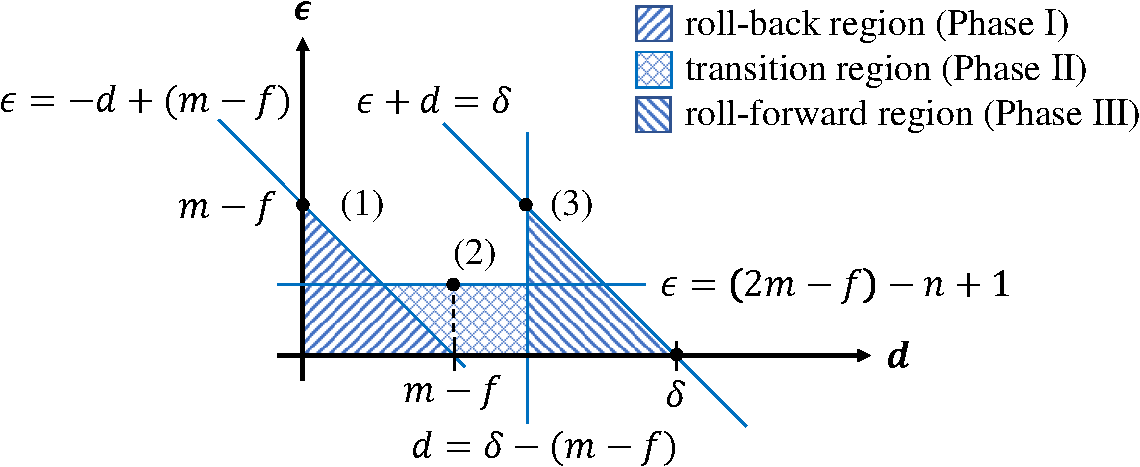
\includegraphics[width=\linewidth]{figures/d-e-space}
  \caption{\protocol/ steps in a $d-\epsilon$ space. A point $(d, \epsilon)$
means one step to update $\epsilon$ chunks when $d$ chunks have been updated.
Constraints produce feasible regions (e.g., the left side of the line $\epsilon
= -d + (m - f)$ satisfies $\epsilon \le -d + (m - f)$, which is
Inequality~\ref{eq:roll-back-constraint}). Points (1) -- (3) represent three
steps of a write path. \vspace{-1em}}
  \label{fig:d-e-space}
\end{figure}

In Figure~\ref{fig:d-e-space}, we color all feasible $(d_i, \epsilon_i)$ points
that satisfy the constraints. The left triangle region always supports
roll-back in \emph{any distribution} of failures, because any point/step
therein can survive the most adversarial case which leads to
Inequality~\ref{eq:roll-back-constraint}. Similarly, any point/step in the right triangle region is
constantly recoverable by roll-forward. Between them may exist a
\emph{transition region} where we cannot say for sure whether recovery will be via rolling forward or backward. 
One or the other will surely work, and the exact choice depends on the failure distribution (particularly, the choice of $f_1$ as
discussed for Inequality~\ref{eq:discretionary}).

Having the model and constraints, we now solve the optimization problem: find the
maximum $\delta$ so that there is a safe write procedure.  A write procedure is
safe as long as every step is recoverable, i.e., located in the
feasible regions in Figure~\ref{fig:d-e-space}.  As long as $\epsilon = (2m -
f) - n + 1 \ge 1$, i.e., $n \le 2m - f$, all three regions connect. That means
any step can find a feasible $\epsilon$ until $d = \delta$ which is the end of
a write path. If so, there is no safety restriction on the value of $\delta$,
which can be up to $u$.

Otherwise, when $n > 2m - f$, the transition region is empty. But if the
roll-back region and the roll-forward region connect, a write path 
always exists. Thus, we need
$\delta - (m - f) \le m - f$, i.e., $\delta \le 2(m
- f)$. All in all, the maximal $\delta$ is as follows.
\begin{equation}
\delta_{\max} =
\begin{cases}
u, & \text{if } n \le 2m-f;\\
\min\{2(m-f), u\}, & \text{otherwise.}
\end{cases}
\label{eq:delta}
\end{equation}

Next, we determine other parameters of
Algorithm~\ref{alg:write}. As Figure~\ref{fig:d-e-space} shows, when $d = 0$,
we take the first step. To reduce the overall latency, we update as many chunks
as possible in parallel. Hence, $s_1$ should be $m-f$.  As a result,
this step will reach from $d=0$ to $d=m-f$, bypassing the entire roll-back region. This
step corresponds to Phase~\Romannum{1} in Algorithm~\ref{alg:write}. Then, we
go through the transition region where $\epsilon = (2m - f) - n + 1$.
Different from a triangle-shaped region, it is possible we need more than one
step to get across the region. These steps make Phase~\Romannum{2}. Finally, we
can go through the roll-forward region in a single step with $s_3=m-f$ in
Phase~\Romannum{3}. In conclusion, \protocol/ produces a safe write procedure
whose every step is recoverable, with maximum $\delta$ as well as minimal latency.

We condense the above findings into the following theorem on the necessary
data redundancy in \protocol/.

\emph{FAW Theorem -- Let P be a write protocol for a $k$-of-$n$ fault tolerance
scheme with $m$ redundant chunks per stripe. Consider a write of $u$
chunks (\emph{including} redundant chunks) of a stripe. If P guarantees crash
consistency and tolerates up to $f$ chunk failures ($f \le m$) during the
write, then P must have the following data redundancy, i.e., an additional
version of $v$ chunks such that:}
\begin{equation}
v \ge
\begin{cases}
  0 & \text{if } n \le 2m-f;\\
  \max\{u - 2(m - f), 0\} & \text{otherwise.}
\end{cases}
\label{eq:v}
\end{equation}

Proof of the theorem is straightforward. As $\delta = u - v$ by definition,
substitute $u - v$ for $\delta$ into Equation~\ref{eq:delta}. The equation
translates to $v_{\min} = 0$ if $n \le 2m - f$, or $v_{\min} = \max\{u - 2(m - f), 0\}$
otherwise. That is exactly the meaning of Inequality~\ref{eq:v}.

\vspace{-1em}
\subsection{Multi-Stripe Write}
\vspace{-0.5em}

An atomic write request may modify data across multiple stripes. Those physical
stripes can be \emph{conceptually} viewed as one stripe for performing
\protocol/. Particularly, the $i$th chunk of the conceptual stripe consists of
the $i$th chunk of every physical stripe. For example, a write modifies D$_1$
of Stripe~1 and D$_2$ of Stripe~2. Then, \protocol/ runs as if Stripe~1 and
Stripe~2 are one stripe, whose D$_i$ is a conceptual combination of the D$_i$
of Stripe~1 and the D$_i$ of Stripe~2. Accordingly, the write request is
regarded as updating both D$_1$ and D$_2$ of the conceptual stripe. In such a
view, the write procedure requires no change to handle the write request.
Note that we actually only update the modified physical chunks, so this
approach does \emph{not} introduce any extra chunk write.

% In practice, chunks are typically organized in a more complex way than a
% simple stripe. Take RAID~\cite{SNIA:RAID} for example.
% Figure~\ref{fig:stripe-depth} depicts the concept of \emph{depth}. Data
% chunks~0--23 are not directly striped.  Instead, they are grouped and the
% groups are striped. The size of a group is the depth of a stripe. A write
% request may update chunks in multiple stripes.

% Those variant data layouts can be viewed conceptually as a \emph{virtual
% stripe} when performing \protocol/. Let's assume all blue chunks in
% Figure~\ref{fig:stripe-depth} have to be updated by a write. We can regard
% Stripe~0 and Stripe~1 as a single virtual stripe with \emph{virtual chunks}
% D$_1$--D$_4$ and P. The \protocol/ protocol runs as if D$_1$, D$_2$, D$_4$ and P are
% to be updated. But when updating a virtual chunk, we only need to update the
% modified physical chunks, so this approach does \emph{not} introduce any extra
% update.
%
% \begin{figure}[!ht]
%   \centering
%   \includegraphics[width=\linewidth]{figures/stripe-depth}
%   \caption{Example data organization of two stipes with depth=4. Blue chunks
% are updated by a single write request.}
%   \label{fig:stripe-depth}
% \end{figure}

\vspace{-1em}
\subsection{Versioning and Recovery}
\vspace{-0.5em}

A write procedure may modify one or more chunks (belonging to one or more
stripes, respectively) on a storage node. It writes a version record for the
chunk(s) to such a node before it updates the chunk(s).

On recovery, we can tell the version of a chunk from its version record. First,
we guarantee that a version record is persistent \emph{before} its
corresponding chunk writes are performed. Therefore, having no version record
implies that the chunk is \emph{not updated}. Second, a version record holds
the phase number of its corresponding chunk writes. That means, if the maximum
phase of any found record is $p$, any other chunk of Phase~$q$, where $q<p$,
must be \emph{already updated}, but Phase~$p$ is regarded as corrupted. Third,
a version record also includes all other chunks that are \emph{intended to be
updated} by the write.  All in all, we can infer the version of a chunk in the
following way. If a chunk is not updated and also not intended to be updated,
it does not change in the write, so its content is both old-version and
new-version; if a chunk is not updated but intended to be, it contains
old-version data; if a chunk is updated, it simply contains new-version data;
otherwise, the chunk is regarded as without any valid version.

Although the recovery policy (roll-back or roll-forward) for each phase or
failure distribution varies, the actual recover procedure is \emph{unified} and
simple. We only need to count the number of old-version and new-version chunks
as specified above, and then recover the version that has more chunks. If that
version still has not enough chunks to recover, the number of failures must be
beyond $f$, so that we should do failover with any detected fault and retry the
write; otherwise, \protocol/ guarantees that the version is recoverable.

\vspace{-1em}
\subsection{Discussion: Relaxing Fault Tolerance}
\vspace{-0.5em}

We distinguish $m$ and $f$ in the protocol. Note that this implies a tradeoff between
storage cost and fault tolerance. We relax fault tolerance during the write
path to gain storage cost savings, which leads to reduced network traffic,
improved I/O performance, and extended NVM endurance. This is a conscious
design choice, for several reasons. \textbf{(1)}~We only reduce fault tolerance
of a \emph{tiny} fraction of data.  Suppose 128 threads each writing 4 pages of
1~TB data. Only 0.0002\% data is temporarily weakened in terms of fault
tolerance. The remaining 99.9998\% keeps the original fault tolerance level.
\textbf{(2)}~\protocol/ offers the flexibility to precisely specify and control
the desired degree of fault tolerance relaxation. It should be up to users to decide
the tradeoff. As far as we know, \protocol/ is the first protocol to
\emph{explicitly} differentiate fault tolerance levels in read and write paths,
while many existing systems already \emph{implicitly} sacrifice fault tolerance
for performance.  For example, a battery-backed DRAM that logs in-progress writes
in a high-end RAID card~\cite{Denehy:2005:JRS:1251028.1251035} is less
fault-tolerant than the underlying group of SSDs. Also, the reality is that not
all components are equally fault tolerant in a distributed
system~\cite{Ford:2010:AGD:1924943.1924948}.  \textbf{(3)}~With \protocol/, a
write failure is not silent, and recoverable by an upper-layer \emph{retry}
mechanism (e.g., as used in Google File
System~\cite{Ghemawat:2003:GFS:945445.945450}). A seamless
failover~\cite{5388891, 6136239} can be supported by reserving spare storage
nodes. Retry is especially helpful when $f=0$ (for RAID~4/5).  But
in most cases (replication, RAID~6+ and erasure coding), $m$ is large enough to
enable a reasonable $f$.

% We add to the RAIN controller a special fast \emph{non-volatile} cache (e.g.,
% STT-RAM)~\cite{Apalkov:2013:STM:2463585.2463589,
% Zhao:2013:KCP:2540708.2540744}, whose write latency can be as low as within
% 20 $\mu$s.
